
%(BEGIN_QUESTION)
% Copyright 2010, Tony R. Kuphaldt, released under the Creative Commons Attribution License (v 1.0)
% This means you may do almost anything with this work of mine, so long as you give me proper credit

Sketch the proper tube connections to calibrate this pneumatic DP transmitter to a range of 0 to 30 inches water column using a manometer as the pressure standard, and a test gauge to sense its 3-15 PSI output:

$$\includegraphics[width=15.5cm]{i03680x01.eps}$$

\underbar{file i03680}
%(END_QUESTION)





%(BEGIN_ANSWER)

This is not the only correct solution.  The manometer connections may be reversed and still function perfectly:

$$\includegraphics[width=15.5cm]{i03680x02.eps}$$

(All-or-nothing grading: either 10 points for a functioning setup, or 0 points if anything is wrong)

%(END_ANSWER)





%(BEGIN_NOTES)

{\bf This question is intended for exams only and not worksheets!}.

%(END_NOTES)

